\chapter{Aufbau \programname}

\section{Architekturbeschreibung}
Im Groben gehalten funktioniert der Daten- und Befehlsfluss im Trufflehog-Entwurf
wie im klassischen MVC, der Presenter aktiviert Services, welche das Model basierend
auf dem empfangenen Netzwerkverkehr verändert und das View aktualisiert sich am Model.
Da viele Threads im Programm parallel durchlaufen aber dennoch kommunizieren müssen,
verlassen wir uns an einigen Stellen auf das \gls{observerpattern} mit einer
Multi-Thread kompatiblen Datenstruktur.\newline
\newline

\section{Paketbeschreibung}

\subsection{command}
\label{subsec:command}
Das command-Package beinhaltet Commands. Ein command ist ein Befehl der auf
dem Model ausgeführt wird. D.h. alle objekt die das Model irgendwie verändern
werden als command gekapselt, sodass deren veränderung auf dem Model
ausgeführt werden kann. Zum Beispiel werden alle empfangene netzwerk\glspl{paket}
und Benutzerbefehle als command gekapselt, da diese direkt das Model beeinflussen
in dem sie bie dem \gls{executor} ankommen und dort ausgeführt werden.
\newline
\newline
Dieses Design hat zwei große Vorteile. Zum einen herscht eine lose Kopplung zwischen
dem der das Model verändern will und dem Model selber, was zur Modularität des ganzen
Programmes beiträgt. Zum anderen kann man die Commands speichern und zu einem
späteren Zeitpunkt auf ein Snapshot des Modelles wieder ausführen um das originale
Model wieder herzustellen. Mehr dazu im
\hyperref[subsubsec:replaylogging]{replaylogging}-Package Weiter bietet dieses
design den großen Vorteil das es hohes erweiterbakeits Potential hat. Zum Beispiel
könnte man relativ einfach eine undo und redo Funktion in ein Command einbauen um
zwischen verschiedene Modelzuständen hin und zurück zu springen. So eine
Funktionalität ist zwar nicht geplannt, aber sie demonstriert wie einfach man so
etwas implementieren könnte.
\newline
\newline
\begin{figure}[H]
  \centering
  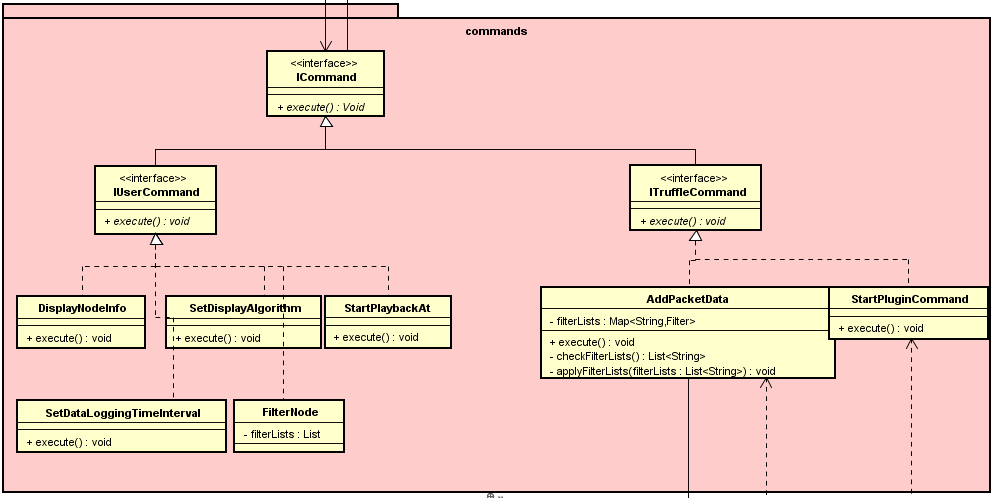
\includegraphics[width=\textwidth]{../diagramimages/commands.png}
  \caption{command-Package}
\end{figure}

Es gibt 2 Arten von Commands, TruffleCommands für die bearbeitung empfangener
Paketdaten, und UserCommands für die Verwaltung der Benutzeroberflächenbefehle.

      \subsubsection{trufflecommand}
      \label{subsubsec:trufflecommand}
      ***TruffleCommands package image goes here***
      \newline
      \newline
      Jegliche empfangene Paketdaten werden zuerst in \glspl{truffle} umgewandelt wie
      im \hyperref[subsubsec:truffleprocessor]{truffleprocessor}-Package erleutert. Dort
      werden die erzeugten \glspl{truffle} in ein Command gesteckt und per Observer Pattern
      wie im \hyperref[subsec:util]{util}-Package beschrieben an alle In­te­r­es­senten verschickt
      (die Listeners).
      \newline
      \newline
      Es gibt nur einen Command Typen für die empfangen Netzwerkpakete, nähmlich den
      AddPacketDataCommand. Diese Entscheidung wurde getroffen um das Programm simple
      zu halten. Commands wie addNode() oder addEdge() sind überflüßig, da diese leicht aus
      einem Netzwerkpaket geschlossen werden können.
      \newline
      \newline
      Der PluginNotRunningCommand wird genau dann verschickt, wenn sich \gls{programname}
      nicht mit \gls{sppname} oder einem äquivalenten Plugin nicht verbinden konnte. Wir
      haben die Funktionalität das \gls{programname} automatisch \gls{sppname} startet
      aufgegeben um die beiden Programme unabhängiger zu gestallten, und um dem Benutzter
      mehr Freiheit zu geben.

      \subsubsection{usercommand}
      \label{subsubsec:usercommand}
      ***UserCommands package image goes here***
      \newline
      \newline

      Wenn der Benutzter eine GUI-Aktion startet die das Model beeinflusst,
      wird ein Command an alle Listener durch das observer pattern wie im
      \hyperref[subsec:util]{util-Package}) beschrieben verschickt. Für jede mögliche
      GUI aktion die das Model beeinflusst gibt es einen passenden Command.

      \subsubsection{queue}
      \label{subsubsec:queue}
      Die  welche beispielsweise der executor besitzt. Es
      sind ggf. mehrere tatsächliche Queues vorhanden, was einen Manager verlangt
      um nach dem Round-Robin-Prinzip faire Verteilung zu ermöglichen.

      *** Bitte jemand anders erleutern, blocking queue idee fehlt etc. ****


\subsection{service}
\label{subsec:service}

Im service package befinden sich alle Prozesse die ihren eigenen Thread haben,
mit ausnahme vom

\begin{figure}[H]
  \centering
  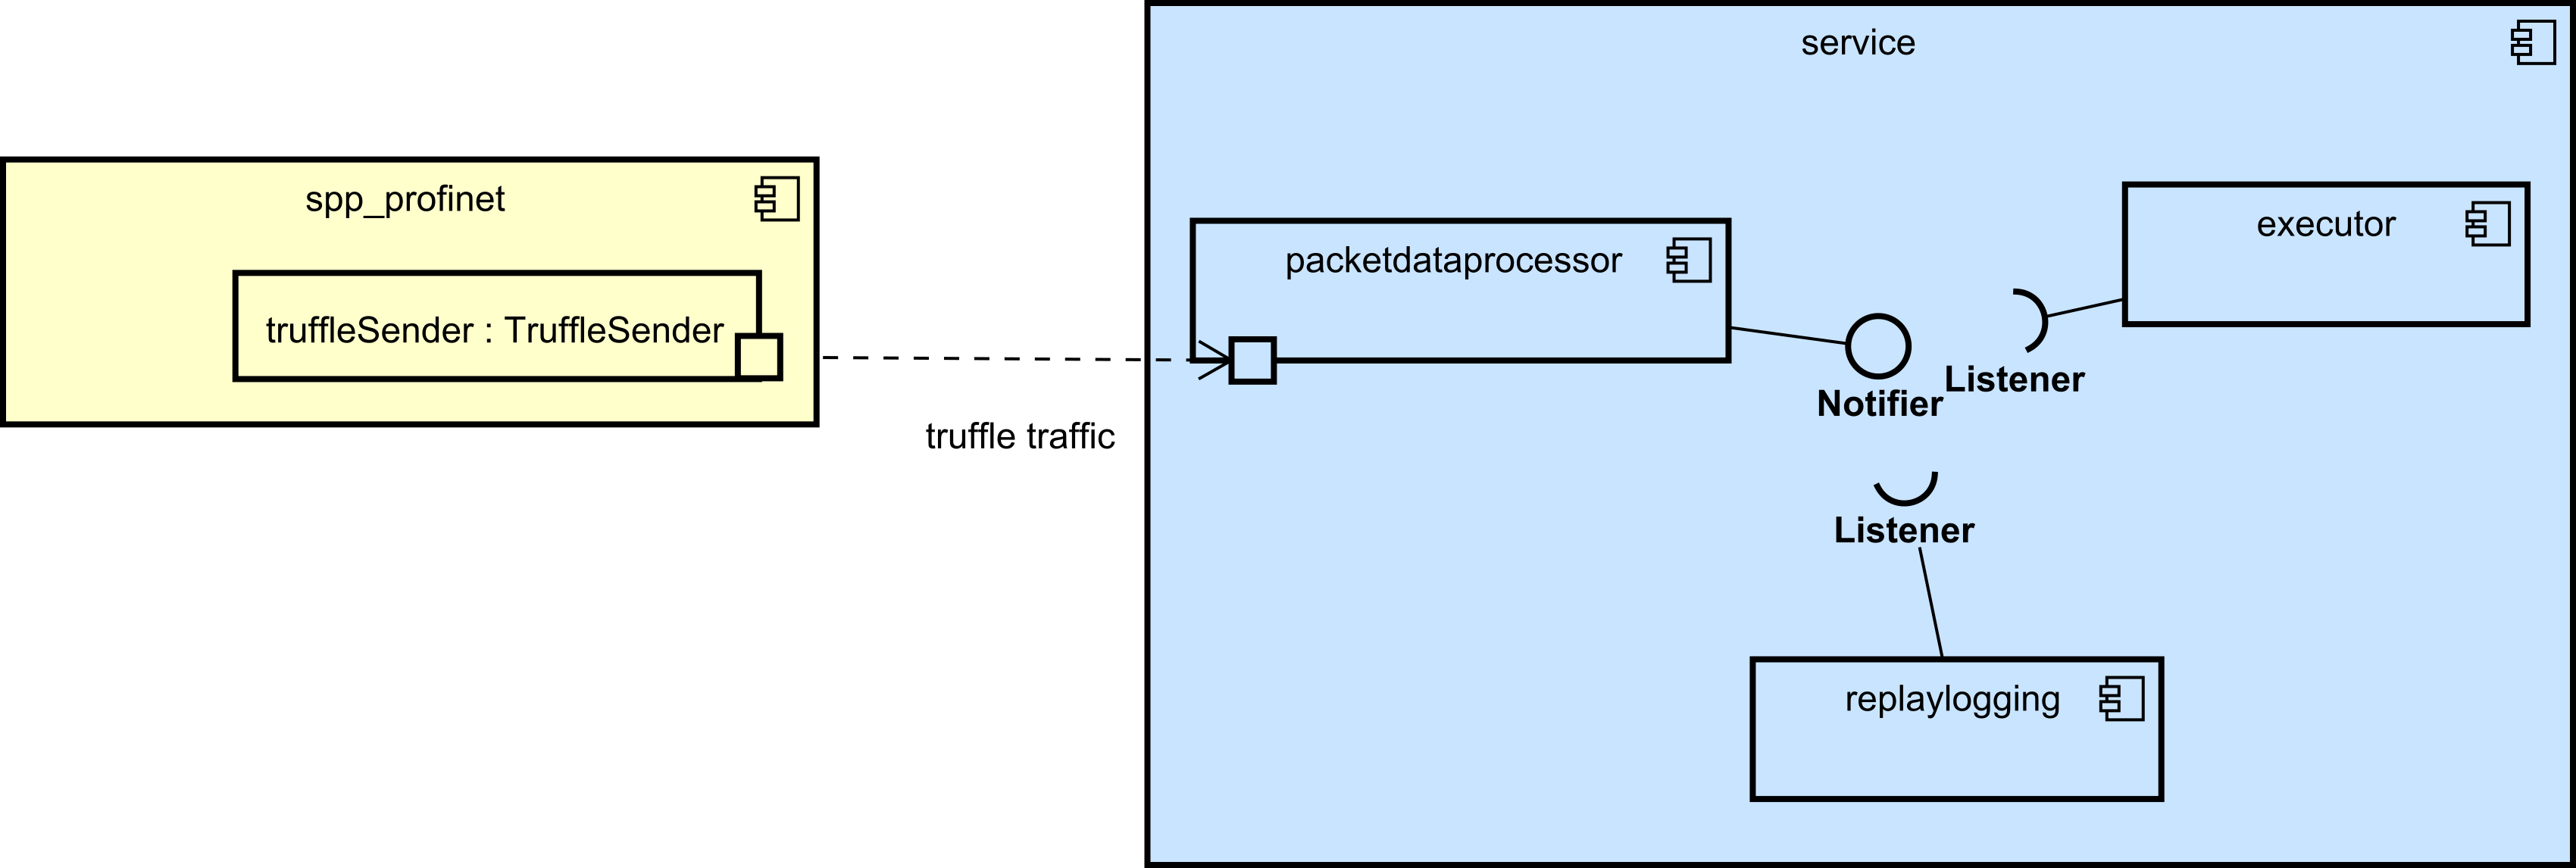
\includegraphics[width=\textwidth]{../diagramimages/service.png}
  \caption{service-Package}
  \medskip
\end{figure}

    \subsubsection{truffleprocessor}
    \label{subsubsec:truffleprocessor}
    Der truffleprocessor ist die Empfangsstelle für die von uns in der
    \gls{ipc} benutzen Truffles. Außerdem erzeugt er die später verwendeten
    Commands und benachrichtigt als \gls{notifier}.

    \subsubsection{replaylogging}
    \label{subsubsec:replaylogging}
    Das datalogging kümmert sich um die gesamte gewünschte
    Speicherung/Loggen und, falls implementiert, die Verfügbarkeit der
    Video-Daten. Es speichert sowohl regelmäßige Snapshots des gesamten
    Graphen, als auch einzelne Commands für eine Schrittweise Rückverfolgung
    des Ablaufes.

    \subsubsection{executor}
    \label{subsubsec:executor}
    Der executor ist das Unterpackage, in welchem die Anwendung bzw.
    Ausführung der Commands stattfindet. Er ist ein \gls{listener} für Commands
    von sowohl dem view-Package als auch dem truffleprocessor.


\subsection{presenter}
\label{subsec:presenter}

Der presenter ist für den Aufbau von \gls{programname}, also das
Initialisieren, Instanziieren und Referenzieren aller Programmelemente zuständig.

\begin{figure}[H]
  \centering
  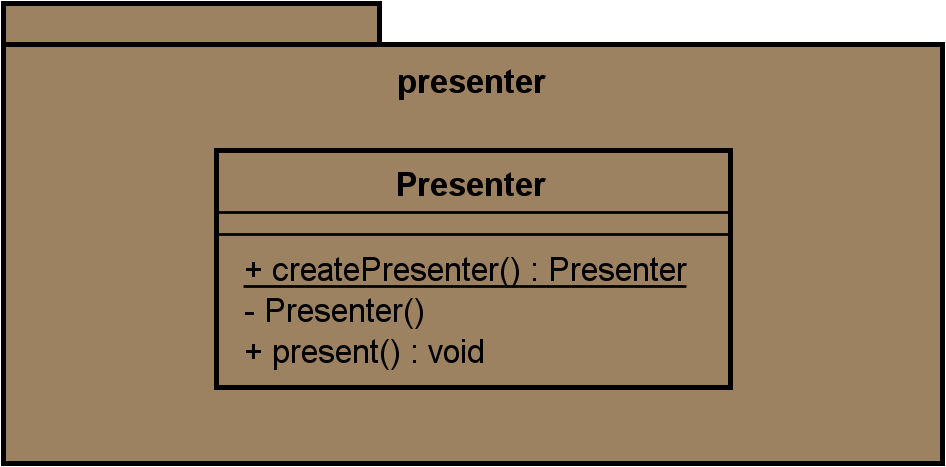
\includegraphics[width=\textwidth]{../diagramimages/presenter.png}
  \caption{presenter-Package}
\end{figure}

Er ist der erste Thread und erzeugt alle weiteren, zum Beispiel einen für jeden
Service. Außerdem liest er aus einer Settings-Datei und stellt das Programm ein.
Das heisst er initialisiert bestimmte Attribute entsprechend. Danach erschöpft
sich die Nützlichkeit des presenter bis zu einem neuen Programmstart.


\subsection{util}
\label{subsec:util}


Unsere Variante des \gls{observerpattern}s.

\begin{figure}[H]
  \centering
  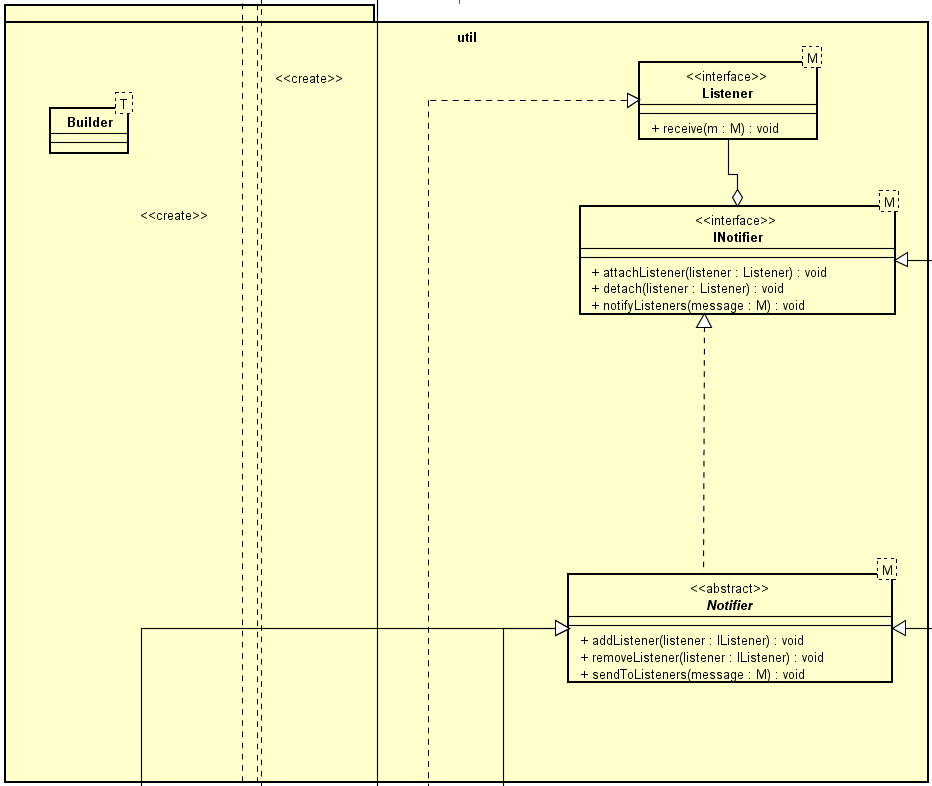
\includegraphics[width=\textwidth]{../diagramimages/util.png}
  \caption{util-Package}
\end{figure}

Da wir sowohl Interfaces als auch Klassen bzw. abstrakte Klassen als
\gls{notifier} haben, kommen wir nicht um eine Modifizierung des klassischen
\gls{observerpattern} herum. Nun haben wir die Möglichkeit sowohl ein
\gls{notifier}-Interface zu erweitern als auch eine abstrakte
\gls{notifier}-Klasse zu beerben. Der \gls{listener} funktioniert genau wie ein
Observer.


\subsection{model}
\label{subsec:model}

Die Hauptdatenstruktur von \gls{programname}: das model-Package.

\begin{figure}[H]
  \centering
  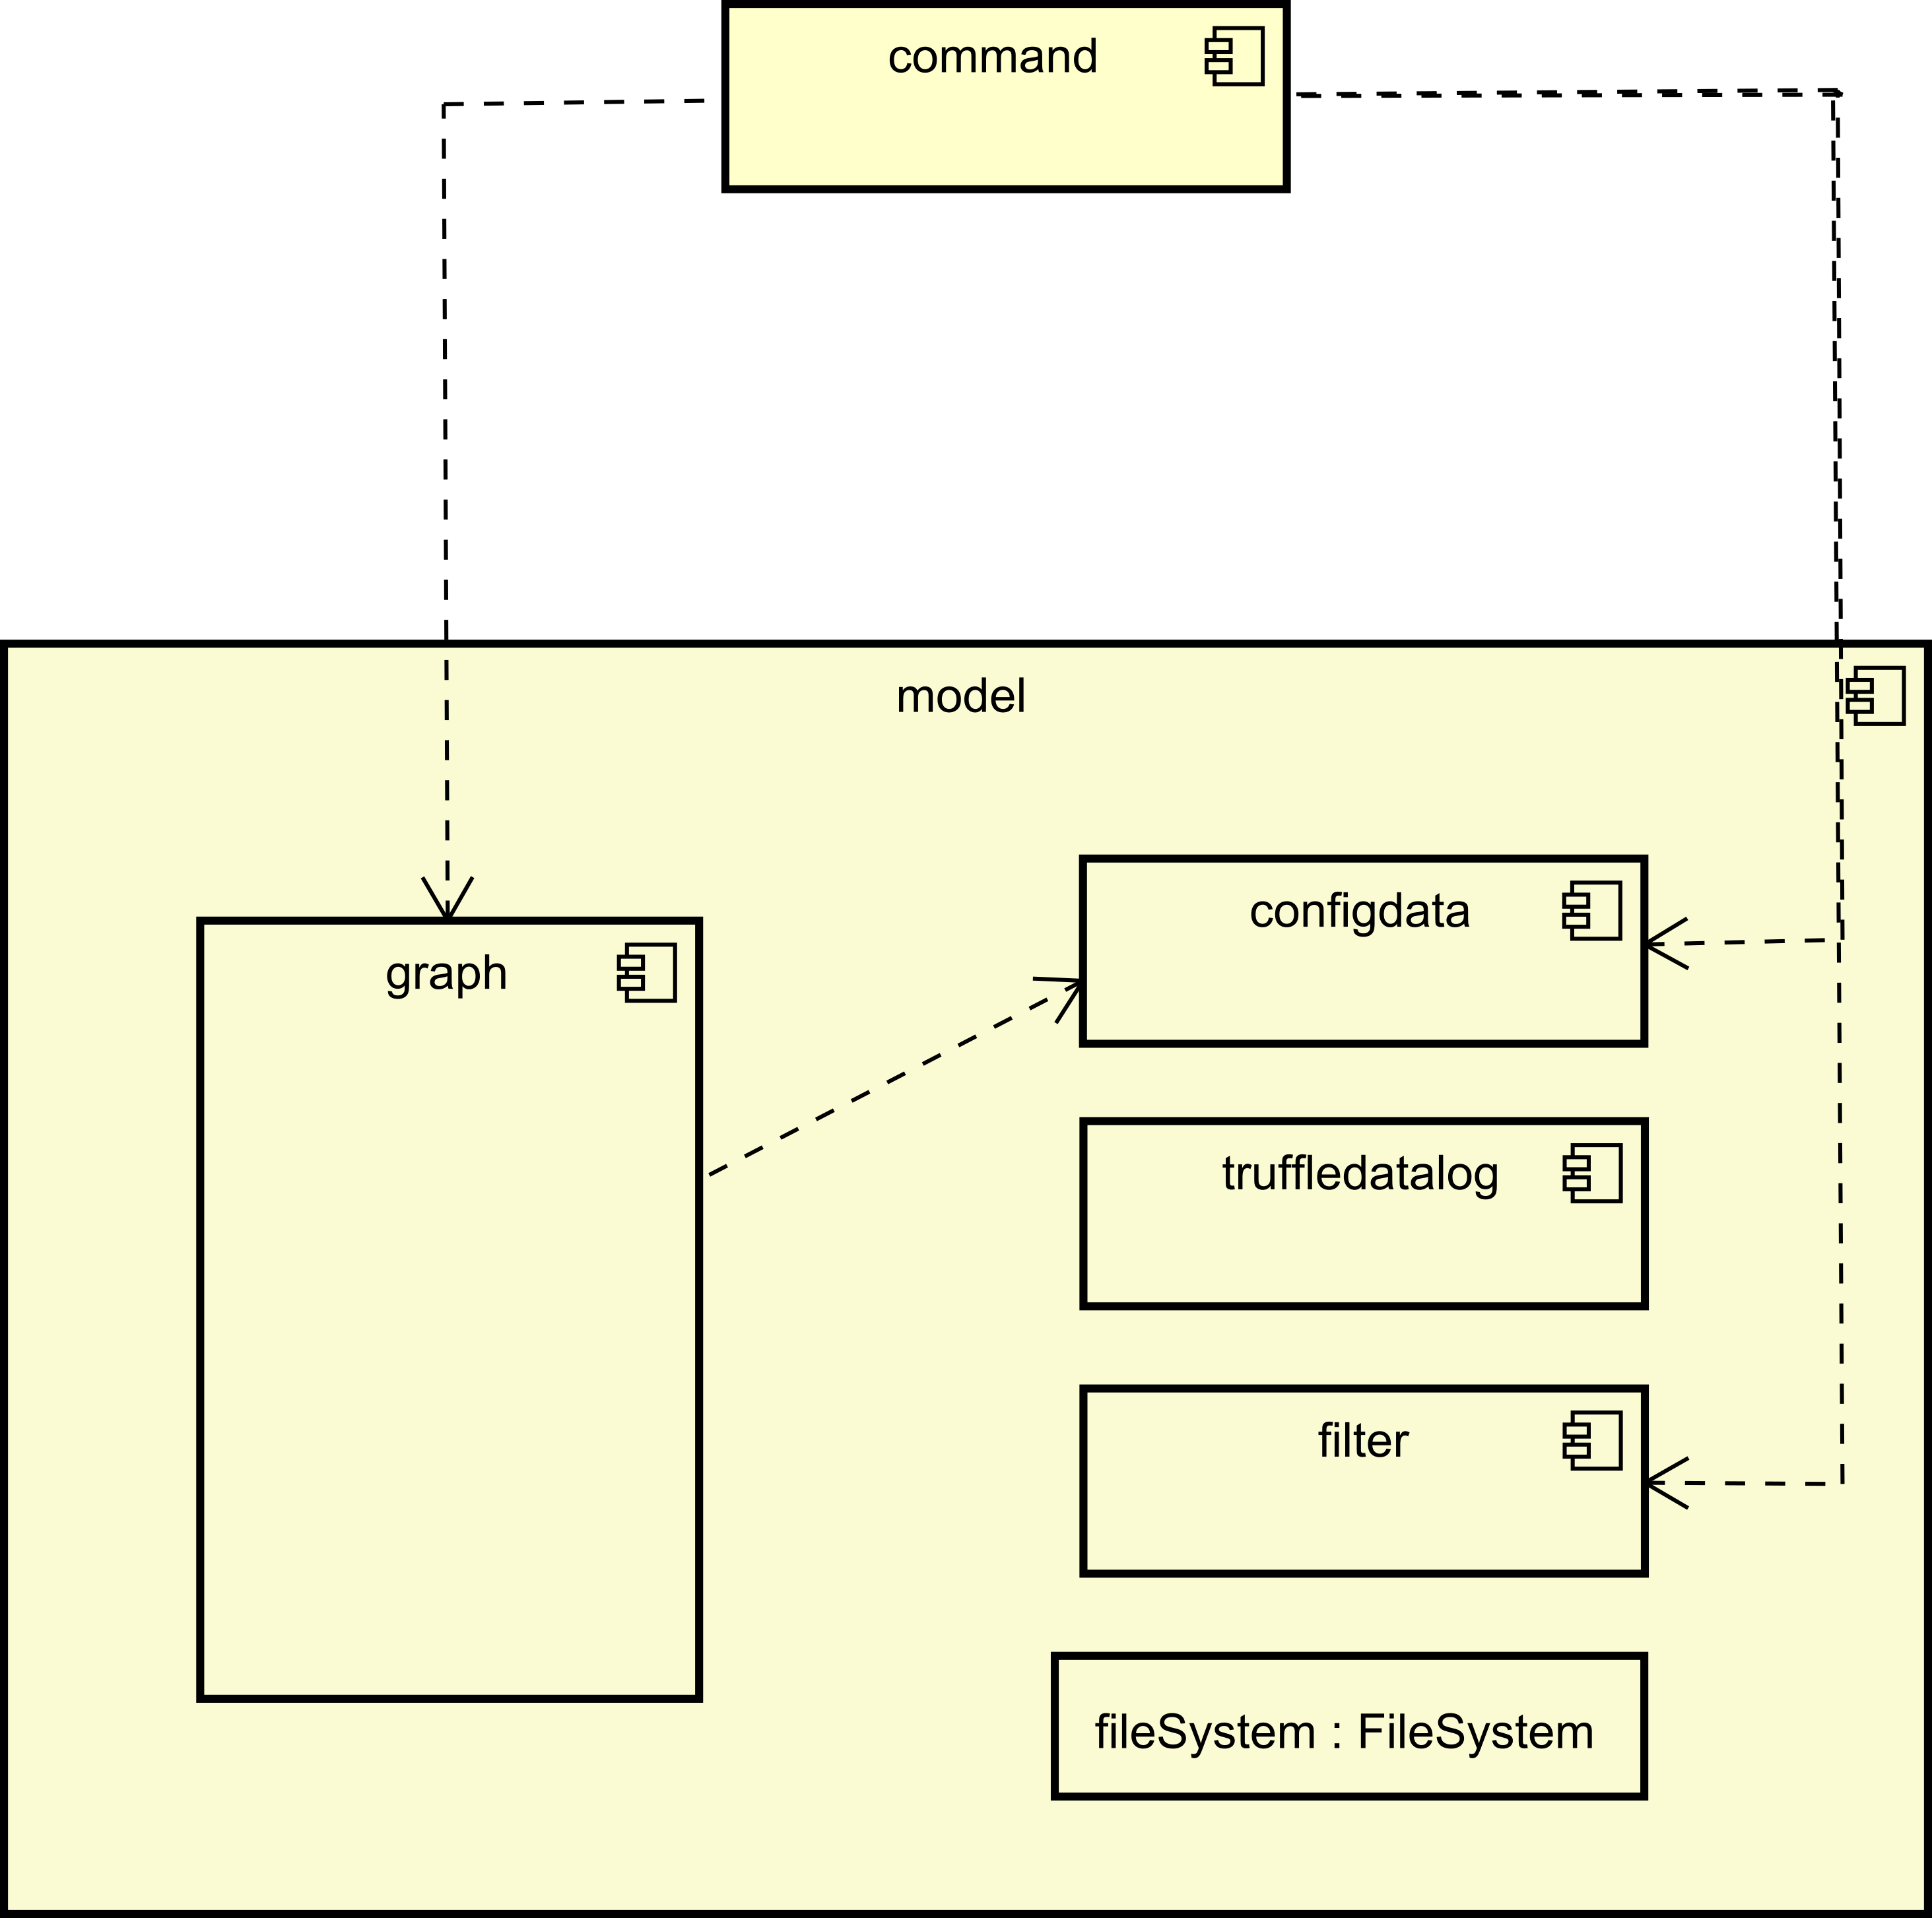
\includegraphics[width=\textwidth]{../diagramimages/model.png}
  \caption{model-Package}
\end{figure}

    \subsubsection{graph}
    Dieses Unterpackage macht das eigentliche Modell aus. Der gesamte Graph sowie all seine möglichen Layouts, entsprechende Interfaces und ein Proxy aus dem \gls{proxypattern} für die Entkopplung sind hier enthalten.
    \subsubsection{filter}

    \subsubsection{settingsdata}

    \subsubsection{graphlog}


\subsection{view}
\label{subsec:view}

\subsection{interactors}
\label{subsec:interactors}
